\chapter{The dependency grammar}
\label{ch:dependecy-grappamr}

The Stanford dependency analysis of a given text constitutes the input for the algorithm developed in the current work. It provides the foundation to build the syntactic backbone used adopted here. This chapter offers an overview of the grammar and the parser developed at the Stanford university. In the last part of the chapter is discussed the cross theoretical connection between the dependency and systemic functional grammars. 

\section{A briefing on the theory of dependency grammar}
Traditionally, Latin language tended to be analysed with the \textit{dependency model} based on theories of what was called \textit{government}. It explains the syntagmatic relations of the subtype Firth called \textit{colligation} (i.e. relations between grammatical categories). Government is a way of explaining the rich inflections of language (such as Latin) in terms of how particular words govern, that is to say, determine, the inflection of other words. \citep[p.66]{McDonald2008}

\citet{Tensiere2015} explains how government works by giving example of Latin text analysis where the inflections immediately give aloto of information about relations between different words. For example the verb agree in person and number with its subject. From this point of view the verb governs the subject. The verb also governs complements and adjuncts which can be seen as relations of dependency between a governing element or controller and a governed element or dependant. It is important to note that Tensiere analysed syntax at the level of clause where he identified a verb node as the main controller. 

Contrary to Latin, languages like English or Chinese, where there is little or most of the time none of the inflectional marking to identify dependency relations, are much harder to analyse in terms of such relations. This was a motivation for Tensiere to reinterpret dependency relation in semantic terms rather than inflectional marking. As \citet{McDonald2008} points out, this can be regarded as extending syntagmatic relations of the clause to include what Firth was calling \textit{collocation} relations (i.e. links between lexical items). Tensiere framed his theory in terms of syntagmatic relations as expressing a model of experience. He compares the verbal node of the clause to a complete little drama. Like a drama, it obligatorily consists of an action, most often actors and features of settings. Expressed in terms of syntactic structure, the action, actors and settings become the verb, participants and circumstances \citep{Tensiere2015}. 

Further, Tensiere explains \textit{categories of language} as \textit{categories of thought}. The human mind shapes the world in its own measure by organising experience into a systematic framework of ideas and beliefs called categories of though. Likewise, the language shapes thought in its own measure by organising it into a systematic framework of grammatical categories \citep{Tensiere2015}. He stresses though, that the latter ones can vary considerably from language to language and that the analysis of syntactic relations shall be carried on not in terms of grammatical categories but rather in terms of functions. He explain through an example that analysis in terms of nouns and verbs i.e. grammatical categories, tells nothing about the tie that links the words, whereas if we turn to notions such as subject and complement it all of the sudden becomes clear: the connections are established, the lifeless words become a living organism and the sentence take on a meaning \citep{Tensiere2015}.

\section{Stanford dependency grammar (and parser)}
Dominant \citet{Chomsky1981} theories define grammatical relations as configurations of \textit{phrase structure} representations, which is nesting of multi word constituents. Other theories such as Lexical-Functional Grammar reject the adequacy of such an approach \citep{Brensan2000} and advocate a functional representation for syntax.

When motivating its stance, \citet{Marneffe2006} insists on practical rather than theoretical concerns proposing that structural configurations be defined as grammatical roles (to be read as grammatical functions)\citep{Marneffe2006}. For example she insists that, information about functional dependencies between words grants direct access to the predicate-argument relations which are not readily available form the phrase structure parses and can be used off the shelf for real world applications. She avoids going into theoretical debates and focuses on the suitability of the grammar for parsing within the context of relation extraction, machine translation, question answering and other tasks.

The functional dependency descriptions is precisely the aspect which makes possible the link between the Stanford Dependency Grammar and Systemic Functional Structures targeted in the current thesis. 

%\section{The dependency set}
The design of Stanford dependency set \citep{Marneffe2006, Marneffe2008,  Marneffe2014, Silveira2014} bears a strong intellectual debt to the framework of Lexical Functional Grammars \citep{Brensan2000}. \citet{Marneffe2006} started designing the relation typology from GR \citep{Carroll1999} and PARK \citep{King2003} schemes following a LFG style and according to the principles described in Generalization \ref{def:design-principles}.

\begin{generalization}[Design principles for Stanford dependency set]\label{def:design-principles}\leavevmode
	\begin{enumerate}
		\item Everything is represented uniformly and some binary relation between two sentence words.
		\item Relations should be semantically contentful and useful to applications.
		\item Where possible, relations should use notions of traditional grammar \citep{Quirk1985} for easier comprehension by users.
		\item The representation should be spartan rather than overwhelming with linguistic details. 
	\end{enumerate}
\end{generalization}

When proposing the Stanford dependency, \citet{Marneffe2006} inherits many relations from Lexical Functional Grammars\citep{Brensan2000} and departs from the sets described by \citet{Carroll1999} and \citet{King2003}. She arranges the grammatical relations into a hierarchy rooted in a generic relation \textit{dependent}. This is then classified into a more fine-grained set of relations between a head and its dependent. 
%TODO continue describing Stanford dependecy set 

\section{Stanford Parser: collapsed-cc output}
\label{sec:collapsed-cc-output}
% describing the cc-collapsed
The Stanford Dependency Parser is capable of generating several types of dependency representations. The most convenient and informative version is Collapsed-CC-processed. This structure is created after the initial parse is ready and constitutes a simplified and more intuitive representation of the dependency parse. The collapsed form concerns prepositions, conjunctions and relative clause referents. Dependencies involving prepositions and conjunctions are transformed from basic form in Figure \ref{fig:prep-transf1} to the form where preposition are embedded into the edge relation, as in Figure \ref{fig:prep-transf2}. Similar transformation is done for conjunctions. 

\begin{figure}
	\centering
	\begin{minipage}[b]{0.45\textwidth}
		\centering
		\begin{dependency}[dep-style]
			\begin{deptext}[]
				based \& in \& Luxembourg\\
			\end{deptext}
			\depedge{1}{2}{prep}
			\depedge{2}{3}{pobj}
		\end{dependency}
		\caption{Basic(uncollapsed) preposition dependency}
		\label{fig:prep-transf1}
	\end{minipage}
	\quad
	\begin{minipage}[b]{0.45\textwidth}
		\centering
		\begin{dependency}[dep-style]
			\begin{deptext}[]
				based \& in \& Luxembourg\\
			\end{deptext}
			\depedge{1}{3}{prep\_in}
		\end{dependency}
		\caption{Collapsed preposition dependency}
		\label{fig:prep-transf2}
	\end{minipage}
\end{figure}

Besides collapsing prepositions and conjunctions the DG is further processed to introduce more relations (i.e. connections) even if they break the tree structure. For example the \textit{ref} relation does not appear in the basic dependency structure in figure \ref{fig:rel-transf1} but it appears in the processed dependency structure forming a cycle with \textit{rcmod} and \textit{subjpass} relations.

\begin{figure}
	\centering
	\begin{minipage}[b]{0.45\textwidth}
		
		\begin{dependency}[dep-style-narrow]
			\begin{deptext}[]
				Nina \& , \& who \& is \& coming \& tomorrow\\ % \& , \& makes \& ... \\
			\end{deptext}
			\depedge[edge unit distance =2.2ex]{1}{5}{rcmod}
			\depedge{5}{3}{nsubjpass}
			\depedge{5}{4}{auxpass}
			\depedge{5}{6}{tmod}
		\end{dependency}
		\caption{Basic(uncollapsed) preposition dependency}
		\label{fig:rel-transf1}
	\end{minipage}
	\quad
	\begin{minipage}[b]{0.45\textwidth}
		\centering
		\begin{dependency}[dep-style-narrow]
			\begin{deptext}[]
				Nina \& , \& who \& is \& coming \& tomorrow\\ % \& , \& makes \& ... \\
			\end{deptext}
			\depedge[edge unit distance =2.2ex]{1}{5}{rcmod}
			\depedge{1}{3}{ref}
			\depedge{5}{3}{nsubjpass}
			\depedge{5}{4}{auxpass}
			\depedge{5}{6}{tmod}
		\end{dependency}
		\caption{Collapsed preposition dependency}
		\label{fig:rel-transf2}
	\end{minipage}
\end{figure}

Relations like \textit{ref} introduce cycles but add valuable information useful in various stages of further processing. However, ensuring a tree structure in important for the CG creation stage because it is based on a top down traversal. This is taken care of in the preprocessing stage described in the next stage.

\section{Penn part-of-speech tag set}
In traditional grammar \textit{word classes} or \textit{parts of speech} are a commonly accepted concept. However in SFL, it plays rather an orientation or an approximation role, precisely because the part of speech do not have one to one correspondence to the elements they expound. So terms such as \textit{noun} or \textit{adjective} are useful to denote a class of words that expound a certain element of the structure, but such word class to element correspondences shall by no means treated as definite rules. 
%This is in fact the approach taken in current work and correspondence mappings had between established between part of speech to the set of elements they may expound in various units. %TODO[JB] give examples

Stanford dependency parser starts creation of the parse structure process from the list of tokens annotated with Penn part-op-speech tags. Embedded into the dependency graph, these tags are the part of the syntactic context from which SFG constituency graph is built. 

The Penn tagset was developed to annotate the Penn Treebank corpora \citep{Marcus1993}. It is a large, richly articulated tagset that provides distinct coding for classes of words that have distinct grammatical behaviour.

It is based on the Brown Corpus tagset \citep{Kucera1968} but differs in several ways from it. First, the authors reduced the lexical and syntactic redundancy. In Brown corpus there are many unique pos tags to a lexical item. In Penn tagset the intention is to reduce this  phenomena to minimum. Also distinctions that are recoverable from lexical variation of the same word such as verb or adjective forms or distinctions recoverable from syntactic structure were reduced to a single tag. 

Secondly the Penn Corpus takes into consideration the syntactic context. Thus the Penn tags, to a degree, encode the syntactic functions when possible. For example \textit{one} is tagged as NN (singular common noun) when it is the head of the noun phrases rather than CH (cardinal number). 

Thirdly Penn POS set allows multiple tags per word, meaning that either it cannot be decided or the annotators may be unsure of which one to choose.  

There are 36 main POS and 12 other tags in Pen tagset. A detailed description of the schema, the design and principles and annotation guidelines are described in \citep{Santorini1990}. 

\section{Cross theoretical bridge from DG to SFL}
\label{sec:cross-theoretical-bridge}
\label{sec:dependecy-relations-sfl}

The concept of dependency between pairs of words is long acknowledged in linguistic communities. In traditional terms dependencies are treated as \textit{hypotactic expansions} (see Definition \ref{def:taxis}) of word classes (or parts of speech) where the expanded word acts as \textit{heads} and expanding ones as \textit{dependent} establishing parent-daughter structural relations illustrated in Figure \ref{fig:dependecy-dg}.
%and the description of \citet[pp. 438 -- 443]{Halliday2013}


%\todo{Next I will describe an example of two structures side by side and show how correspondences between the two can be established.}
%\subsection{The nature of dependency}

% head modifier discussion
%\todo{review, new title, talk about , present comparison between parent-daughter and orthogonal/sister dependecy within constituents}

In SFL community the concept of dependency is less salient than the foundational role it plays in the Dependency Grammars. Dependencies are regarded as orthogonal relations between sibling elements of a unit (Figure \ref{fig:dependecy-sfg}) and link the \textit{heads} to their \textit{modifies} in by Hallidayan \textit{logical structure}\citep{Halliday2013}. 

%Within dependency structure the relation is defined as \textit{parent-daughter dependency} while SFL constituency structure the relation is of \textit{sibling dependency}. 

Figure \ref{fig:dependency-relations} illustrates side by side the parent-daughter and sibling dependency relations. In Figure \ref{fig:dependecy-dg} dependency are the only relations between the units of structure whereas in Figure \ref{fig:dependecy-sfg} there are multiple levels (ranks) of units and the dependency relations are relevant only between siblings at the same level within the structure of an unit. SFL regards dependency relations holding only between elements of a unit whereas the relations that connect the units of lower and higher rank are \textit{constituency relations}. Yet when we look at the two structures they resemble in a way each other and next I show how. 

\begin{figure}[hbtp]
	\centering
	\begin{subfigure}{.5\textwidth}
		\centering
		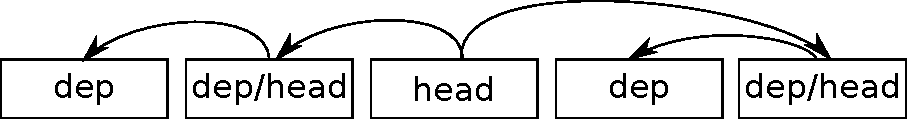
\includegraphics[width=0.9\textwidth]{Figures/SFL-grammar/dependency-dg.pdf}
		\vspace{+22pt}
		\caption{The parent-daughter relations in DG}
		\label{fig:dependecy-dg}
	\end{subfigure}%
	\begin{subfigure}{.5\textwidth}
		\centering
		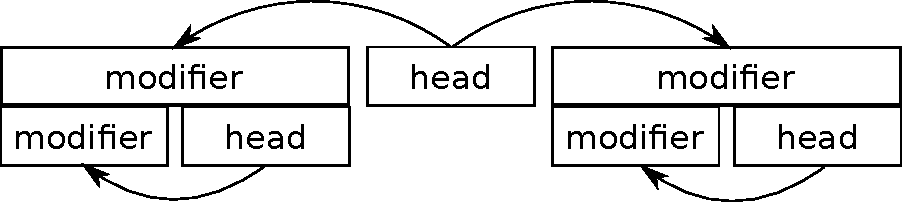
\includegraphics[width=0.9\textwidth]{Figures/SFL-grammar/dependency-sfg.pdf}
		\caption{The head-modifier relations in SFG}
		\label{fig:dependecy-sfg}
	\end{subfigure}
	\caption{The dependency relations in DG and SFG}
	\label{fig:dependency-relations}
\end{figure}

In a nutshell, the parent-daughter dependency relations in dependency grammar unpack into multiple function in systemic functional grammar and specifically it is the head-modifier indirect relation, unit-element componence relation and the head of unit a ``representativeness'' function. 

This difference implies that, when translated to a constituency unit (described in Section \ref{sec:creation-constituency-graph}), the dependency unit, stands for both a unit and that unit's head element. In other words a DG node corresponds to two functional elements at different rank scales. For example the root verb in dependency graph corresponds to the clause node and the lexical item which fills the Main Verb of the clause. By analogy, the head noun of a Nominal Group anchors the entire unit (as a group) and fills the head element of the group. 

\begin{table}[ht]
	\centering
	\begin{tabular}{|l|c|c|ccc}
		\hline
		\textbf{text}              & \textbf{some}                            & \textbf{very}                     & \multicolumn{1}{c|}{\textbf{small}} & \multicolumn{1}{c|}{\textbf{wooden}}            & \multicolumn{1}{c|}{\textbf{ones}}          \\ \hline
		\textbf{units}    & \multicolumn{5}{c|}{\textbf{Nominal Group}}                                                                                                                           \\ \hline
		\textit{elements} & \textit{Quantifying Determiner} & \multicolumn{2}{c|}{\textit{Modifier}}                & \multicolumn{1}{c|}{\textit{Modifier}} & \multicolumn{1}{c|}{\textit{Head}} \\ \hline
		\textbf{units}    &                                 & \multicolumn{2}{c|}{\textbf{Quality Group}}           & \multicolumn{2}{c}{\multirow{2}{*}{}}                                       \\ \cline{1-1} \cline{3-4}
		\textit{elements} &                                 & \textit{Degree Tamperer} & \textit{Apex}              & \multicolumn{2}{c}{}                   \\ \cline{1-1} \cline{3-4}
	\end{tabular}
	
	
	\caption{SF analysis of Example \ref{ex:small-wooden} (reproduced from Table \ref{tab:example-substructure-analisys-cardiff} )}
	\label{tab:example-substructure-analisys-cardiff-repeated}
\end{table}

\begin{figure}[ht]
	\centering
	\begin{dependency}[dep-style-narrow]
		\begin{deptext}[]
			some/DT \& very/RB \& small/JJ \& wooden/JJ \& ones/NNS \\
		\end{deptext}
		\depedge[edge unit distance =2.2ex]{5}{1}{det}
		\depedge{3}{2}{advmod}
		\depedge{5}{3}{amod}
		\depedge{5}{4}{amod}
	\end{dependency}
	\caption{Dependency analysis for Table \ref{tab:example-substructure-analisys-cardiff-repeated} }
	\label{fig:small-wooden-dependecy}
\end{figure}

%The dependency structure is overloaded with two kinds of meaning


Figure \ref{fig:small-wooden-dependecy} and the Table \ref{tab:example-substructure-analisys-cardiff-repeated} represent the analysis of a nominal group from Example \ref{ex:small-wooden} (``some small very small wooden ones'') in Cardiff grammar and Stanford dependency grammar exhibiting a contrast of the two structures. Consider the dependency relation ``det'' a link between the noun ``ones'' and the determiner ``some''. When translated into SF variant the dependency relation stands within Nominal Group between the Head element (filled by word ``ones'') and the Quantifying Determiner element (filled by the word ``some''). By definition all elements in a unit are equal in the structure so the Head and Quantifying Determiner are siblings. So the items (words) filling those elements are sibling. How is then the dependency relation established? 

In SFL there is the concept of Head and Modifier. There is no direct relationship between them but it is said that what the Modifier modifies is the Head. The relation is not a direct one, the Modifier and Head stand for two different kinds of meaning and what the Modifier modifies is not the Head per se but the referent denoted by the head (and thus construed by the entire unit). It is precisely this modification of the head that is called a (sibling) dependency relation and is seldom mentioned in SFL literature because it is considered implicit and recoverable from the SF constituency structure.

The Head also is the element that anchors the entire unit and plays a constitutive role. In this sense the word ``ones'' realizes not only the Head function (sided with Determiner ``some'') but also anchors the entire unit. The relation between the group and it's elements is one of \textit{componence} (Definition \ref{def:componence}) described in Section \ref{sec:componence}. Yet in the role of unit anchor we cannot say that there is a componence relation between ``one'' and ``some'' because it is merely a proxy to the referent rather than the entire unit. So in this role ``one'' can be said to be standing in a parent-daughter dependency relation to ``some'' incorporating the filling and componence relations.

I just showed how the dependency relation in dependency structure (Figure \ref{fig:dependecy-dg}) can be unpacked into two relations in systemic functional structure (Figure \ref{fig:dependecy-sfg}): sibling dependency considered an indirect relation between Head and Modifier (Logical Metafunction) and parent-daughter dependency between unit anchor and the compounding elements, relation which resembles unit componence but is not. 

Lets look at a second example of two relations ``advmod'' from ``small'' to ``very'' and ``amod'' from ``ones'' to ``small''. The interesting case here is the item ``small'' which is the Head of the Quality Group, it anchors the meaning of the whole group and the Quality group fills the Modifier element within the Nominal group. What is not covered in previous example is that the Apex ``small'' not only is a representative of the entire group but it also is a \textit{representative filler} of the Modifier element within Nominal Group. Using the similar translation mechanism as above, this means that, the incoming dependency needs to be unpacked into three levels: the element within the current group (Modifier), the unit class that element is filling (Quality Group) and finally the head of the filler group (Apex). In fact, to be absolutely correct there is one more level. The elements of a unit are expounded by lexical items, so fourth relation to unpack is the expounding of the Apex by ``small'' word.

In this section I laid the theoretical principle for transforming the dependency structure into systemic functional structure. In practice to achieve this level of unpacking the algorithm requires a bottom up and a top down contextualization in terms of elements of structure within a unit and realised sequence of textual units. This implied that the unpacking needs two traversals, a bottom-up and a top one. More on that and the exact algorithm for the translation is provided in Section \ref{sec:creation-constituency-graph}.

Next follows the chapter on Governance and Binding Theory needed to account for the unrealised, covert (Null) Elements in the syntactic structure. It is also an opportunity to perform a similar theoretical translation exercise (as in this section) from one theory of grammar into another.

%
%\todo{close the chapter}
%
%\explain{the problem of bottom up and top down view on the tree structure, due to the fact that head elements plays two roles: of the unit-class(from above) and head-element(from below)}
%\explain{how it is solved with two traversals in the syntactic parsing chapter}
%
%\section{Discussion}